\frame
{
\frametitle{Resultado}
\framesubtitle{Datos de entrada}
\begin{itemize}
	\item<1-> 2 matrices de $1600\ x\ 1600$.
	\item<2-> Se generaron 2,560,000 números \blue{aleatorios} por cada matriz.
	\item<3-> Contra-parte en C++, \red{sin} paralelismo.
\end{itemize}
}


\frame
{
\frametitle{Resultado}
\framesubtitle{Valores de \texttt{BLOCK\_SIZE}}
\begin{center}
	\tiny{
	\begin{tabular}{|l|c|c|c|c|c|c|c|c|c|c|}
		\hline
		\texttt{BLOCK\_SIZE} & 2 & 4 & 5 & 8 & 10 & 16 & 20 & 25 & 32 & 40 \\\hline
		\texttt{Tiempo [s]}  & 44.009 & 9.27 & 6.521 & 5.139 & 5.991 & 4.659 & 4.499 & 1.986 & 2.002 & 2.087 \\\hline
	\end{tabular}
	}
	\\
	\footnotesize
	\vspace{1cm}
	\begin{tabular}{cc}
		Tiempo en CPU: & 52.881 [s] \\
	\end{tabular}
\end{center}
}

\frame
{
\frametitle{Resultado}
\framesubtitle{Gráfico}
\begin{center}
	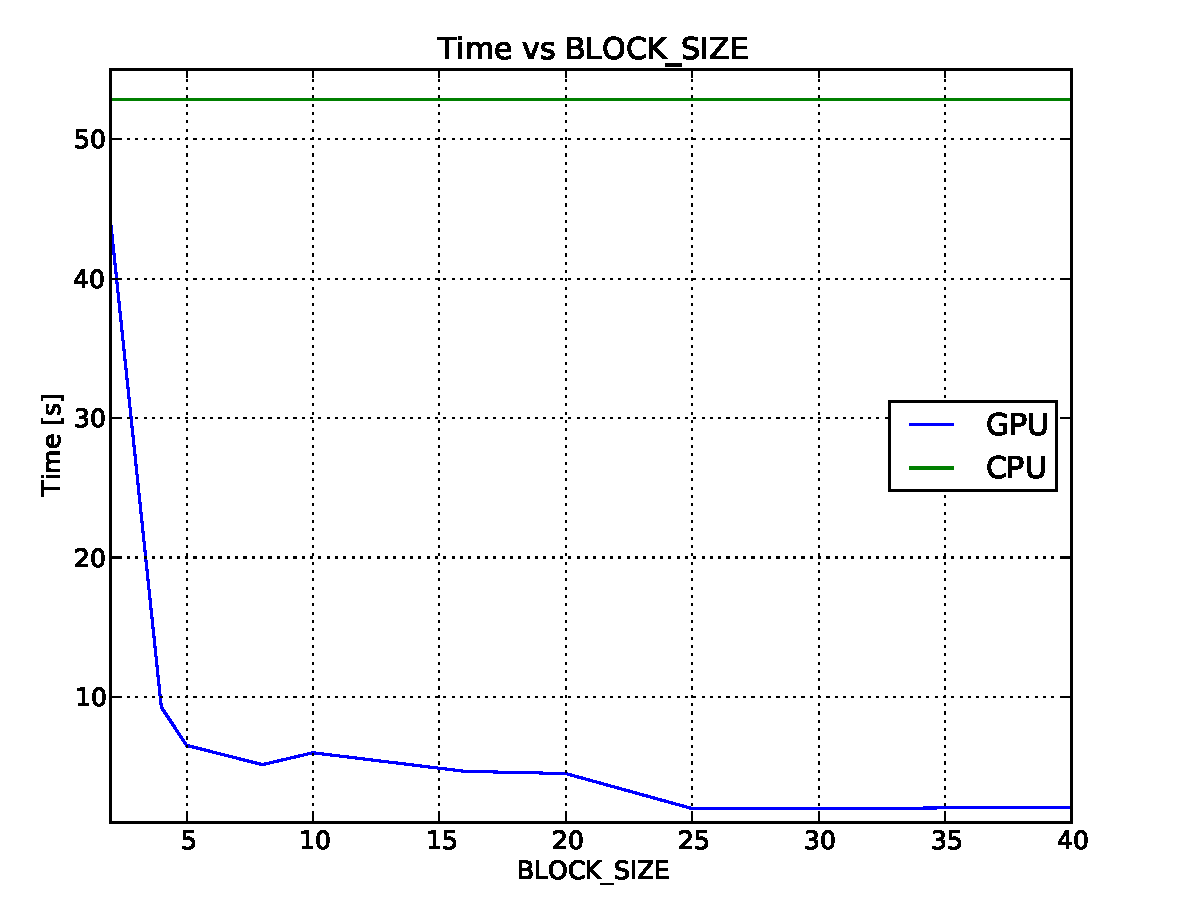
\includegraphics[width=0.8\textwidth]{../doc/img/plot-proyecto.pdf}
\end{center}
}
